\subsection{Experimental Data Overview}

The results are organised around the three research questions introduced in Section~\ref{sec:rq}. The analysis focuses on three main comparison axes: prompt configuration, planning architecture, and model behaviour across scenario configurations. In addition, an exploratory analysis is included for objective sensitivity.

The metrics and experimental conditions are defined in Section~\ref{sec:method_scenarios_models_metrics}. This chapter reports raw shelf deliveries and \gls{llm} calls together with the call-normalised delivery measure defined in Eq.~\ref{eq:deliveries-per-1000-calls}. Raw delivery count remains the main task-completion measure, while the call-normalised value describes deliveries relative to model-interaction frequency. The analyses use matched configuration-level observations drawn from the Calls, Battery + Shelf, and Battery objective families. Repeated executions with the same objective, architecture, prompt configuration, model, and scenario identifiers are averaged before matching, and therefore do not receive additional weight.

\subsection{RQ3: Prompt-Configuration Comparison}
\label{sec:results_prompt_representation}

RQ3 compares collaborative task performance under the tested natural-language and \gls{json}-based prompt configurations. Table~\ref{tab:json_natural_scenario} reports the scenario-level comparison, using 144 matched configuration-level observations for each prompt configuration. Across all six scenarios, the natural-language configuration produced higher mean deliveries and higher deliveries per 1000 calls than the \gls{json}-based configuration.

\begin{table}[H]
\centering
\small
\resizebox{\textwidth}{!}{%
\begin{tabular}{|l|c|c|c|c|}
\hline
\textbf{Scenario} & \textbf{JSON mean del.} & \textbf{JSON del./1000 calls} & \textbf{Natural mean del.} & \textbf{Natural del./1000 calls} \\ \hline
tiny\_balanced\_1v1 & 1.96 & 3.54 & 4.33 & 7.45 \\ \hline
small\_balanced\_2v2 & 0.65 & 1.33 & 3.40 & 4.23 \\ \hline
small\_agv\_heavy\_4v2 & 6.44 & 4.85 & 11.08 & 7.41 \\ \hline
small\_picker\_heavy\_2v4 & 4.90 & 2.85 & 6.60 & 3.88 \\ \hline
medium\_balanced\_4v4 & 4.42 & 2.99 & 8.21 & 4.72 \\ \hline
medium\_agv\_heavy\_6v2 & 3.83 & 2.90 & 9.29 & 7.15 \\ \hline
\end{tabular}
}
\caption{Prompt-configuration comparison by scenario. Each cell summarises 24 configuration-level observations per prompt, matched by objective, planning architecture, model, and scenario.}
\label{tab:json_natural_scenario}
\end{table}

The same overall pattern appears when grouping by model, as shown in Table~\ref{tab:json_natural_model}. The natural-language configuration produced higher mean deliveries and call-normalised delivery values for five of the six models. Phi4 was the exception on both measures, with 5.81 mean deliveries and 8.03 deliveries per 1000 calls under \gls{json}, compared with 5.79 and 7.70 under natural language. The differences were especially pronounced for the two Llama models and Qwen.

\begin{table}[H]
\centering
\small
\resizebox{\textwidth}{!}{%
\begin{tabular}{|l|c|c|c|c|}
\hline
\textbf{Model} & \textbf{JSON mean del.} & \textbf{JSON del./1000 calls} & \textbf{Natural mean del.} & \textbf{Natural del./1000 calls} \\ \hline
llama 1b (3.2) & 0.75 & 0.76 & 2.81 & 2.72 \\ \hline
llama 3b (3.2) & 2.33 & 1.90 & 12.08 & 6.17 \\ \hline
mistral 7b & 4.42 & 3.76 & 7.54 & 4.36 \\ \hline
gemma 12b & 4.21 & 2.60 & 7.69 & 7.16 \\ \hline
phi4 & 5.81 & 8.03 & 5.79 & 7.70 \\ \hline
qwen 14b (2.5) & 4.67 & 4.09 & 7.00 & 6.52 \\ \hline
\end{tabular}
}
\caption{Prompt-configuration comparison by model. Each model and prompt configuration uses $n=24$ configurations matched by objective, planning architecture, and scenario.}
\label{tab:json_natural_model}
\end{table}

These results suggest that the evaluated models were better able to use the natural-language state description than the \gls{json} representation in this implementation. One possible explanation is that converting the simulator state into descriptive sentences made relationships among agents, targets, and constraints more explicit. Although the same state variables were available in the \gls{json} prompt, their meaning had to be inferred from field names, values, and the structure of the object. The natural-language representation may therefore have provided additional linguistic context for models whose pretraining is primarily based on large text corpora.

The result is also consistent with Tam \textit{et al.}~\cite{tam2024letmespeak}, who found that restricting model outputs to structured formats, including \gls{json}, could reduce performance on reasoning tasks. Their study also showed that the effect was task-dependent and that structured formats could remain competitive on classification tasks. In the present experiments, the \gls{json} condition changed both the state representation and the output constraint, so the observed difference cannot be attributed to either factor in isolation. A model trained or post-trained with greater exposure to structured data might behave differently. Moreover, \gls{json} can encode relationships through meaningful field names and hierarchy, but the results indicate that this encoding was less effective than the descriptive representation for the models and planning interface evaluated here.

\begin{figure}[H]
\centering
% Previous raster chart:
% 
\includegraphics[width=0.95\textwidth]{figures/charts/new/delivery_efficiency_prompt_scenarios.png}
\ChartPromptScenarios
\caption{Call-normalised deliveries by prompt format across scenarios. Each bar is calculated from 24 matched configuration-level observations. Higher bars indicate more deliveries per 1000 model calls.}
\label{fig:prompt_efficiency_scenarios}
\end{figure}

\begin{figure}[H]
\centering
% Previous raster chart:
% 
\includegraphics[width=0.95\textwidth]{figures/charts/new/delivery_efficiency_prompt_models.png}
\ChartPromptModels
\caption{Call-normalised deliveries by prompt format across models. Each model and prompt configuration uses $n=24$ matched configuration-level observations. Higher bars indicate more deliveries per 1000 model calls.}
\label{fig:prompt_efficiency_models}
\end{figure}

\begin{figure}[H]
\centering
% Previous raster chart:
% 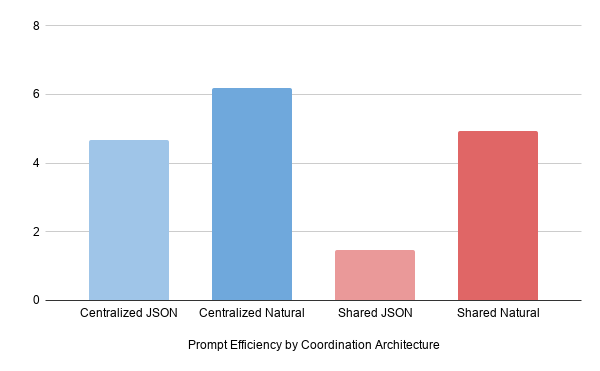
\includegraphics[width=0.82\textwidth]{figures/charts/new/prompt_efficiency_coordination_architecture.png}
\ChartPromptArchitecture
\caption{Call-normalised deliveries by prompt format within each planning architecture. Each bar is calculated from 72 matched configuration-level observations. Higher bars indicate more deliveries per 1000 model calls; the measure describes interaction frequency rather than computational cost.}
\label{fig:prompt_efficiency_coordination_architecture}
\end{figure}

These results show that the tested natural-language prompt configuration, which presented the simulator state in descriptive form, supported better collaborative task performance overall than the tested \gls{json}-based configuration. It produced higher mean deliveries and higher deliveries per 1000 model calls across all six scenario groups and for five of the six models. Phi4 showed a small \gls{json} advantage on both measures. The consistency of the broader pattern supports the answer to RQ3: at the level of the complete prompt configurations, the descriptive natural-language configuration was more effective overall, although the Phi4 result shows that the effect was model-dependent and cannot be attributed to a single formatting component.

\subsection{RQ2: Planning-Architecture Comparison}
\label{sec:results_architecture}

RQ2 compares centralized planning with shared-context per-agent planning. Because shared-context planning can call the \gls{llm} separately for multiple agents, \gls{llm} calls are partly a consequence of the architecture itself. For this reason, the architecture comparison is interpreted primarily through mean deliveries, while the call-normalised value is treated as a secondary measure of model-interaction frequency rather than computational cost.

Table~\ref{tab:central_shared_scenario} reports the scenario-level comparison, with 16 matched configuration-level observations per architecture within each scenario. Shared-context planning produced more mean deliveries in every scenario, although it also made more \gls{llm} calls. Centralized planning therefore used fewer model interactions, while shared-context planning produced higher delivery counts in this dataset.

\begin{table}[H]
\centering
\small
\resizebox{\textwidth}{!}{%
\begin{tabular}{|l|c|c|c|c|}
\hline
\textbf{Scenario} & \textbf{Central mean calls} & \textbf{Central mean del.} & \textbf{Shared mean calls} & \textbf{Shared mean del.} \\ \hline
tiny\_balanced\_1v1 & 605.31 & 3.08 & 717.89 & 6.05 \\ \hline
small\_balanced\_2v2 & 598.54 & 2.67 & 1230.46 & 4.54 \\ \hline
small\_agv\_heavy\_4v2 & 925.89 & 8.67 & 2185.60 & 13.15 \\ \hline
small\_picker\_heavy\_2v4 & 939.61 & 3.86 & 2551.91 & 8.93 \\ \hline
medium\_balanced\_4v4 & 1297.57 & 7.83 & 2412.21 & 8.18 \\ \hline
medium\_agv\_heavy\_6v2 & 816.61 & 7.69 & 1852.57 & 10.59 \\ \hline
\end{tabular}
}
\caption{Planning architecture comparison by scenario. Each architecture--scenario cell summarises 16 configuration-level observations matched by objective, prompt configuration, model, and scenario.}
\label{tab:central_shared_scenario}
\end{table}

The model-level architecture comparison uses 12 matched configuration-level observations per architecture for each model. Shared-context planning produced more mean deliveries for the Llama models, Mistral, Gemma, and Phi4, while Qwen produced more under centralized planning. The delivery gap between the two architectures generally narrowed among the larger selected models, with Qwen reversing the overall pattern. This indicates that the best planning architecture may depend on both model behaviour and scenario size.

One possible explanation for the overall shared-context advantage is that each model call selects an action for only one agent. This may reduce the number of simultaneous decisions that must be produced and avoids requiring the model to construct a mutually compatible joint action in a single response. Centralized planning nevertheless receives the complete shared state and, in principle, can account for dependencies among all agents directly. The results show that access to global information alone did not produce higher delivery performance under the centralized prompt used here; the model also had to integrate that information successfully into a joint plan.

\begin{figure}[H]
\centering
% Previous raster chart:
% 
\includegraphics[width=0.95\textwidth]{figures/charts/new/centralized_shared_deliveries_scenario.png}
\ChartArchitectureScenarios
\caption{Centralized and shared-context mean deliveries by scenario. Each bar is the mean of 16 matched configuration-level observations per architecture and scenario.}
\label{fig:centralized_shared_deliveries_scenario}
\end{figure}

\begin{figure}[H]
\centering
% Previous raster chart:
% 
\includegraphics[width=0.82\textwidth]{figures/charts/new/centralized_shared_deliveries_model.png}
\ChartArchitectureModels
\caption{Centralized and shared-context mean deliveries by model. Each bar is the mean of 12 matched configuration-level observations per architecture and model.}
\label{fig:centralized_shared_deliveries_model}
\end{figure}

Across the selected model artefacts ordered by nominal parameter size, the delivery difference between shared-context and centralized planning generally narrowed, and Qwen reversed the pattern by producing more deliveries under centralized planning. This trend is compatible with the hypothesis that some models handle the additional joint-planning demand more effectively. Related work has reported stronger performance from a larger backbone in planning-based logical reasoning~\cite{zhao2023explicitplanning}, while evaluations of autonomous language-model planning have also found substantial differences between models and identified the strongest tested model as the best performer, although its absolute success rate remained limited~\cite{valmeekam2023planning}. These findings support treating planning capability as model-dependent, but they do not establish parameter count as the cause of the present architecture differences because the evaluated models also differ in model family and post-training. Across the full architecture comparison, shared-context planning produced higher mean deliveries in all six scenario groups and for five of the six selected models. The consistency across different layouts, agent populations, and role balances indicates that this advantage was not restricted to one type of collaboration demand. RQ2 therefore reveals a trade-off: shared-context planning generally produced higher delivery performance in the tested setting, whereas centralized planning required fewer model interactions; the narrowing model-level gap and Qwen reversal show that the preferred architecture remains model-dependent.

\subsection{RQ1: Model Choice and Scenario Complexity}
\label{sec:results_model_choice}

RQ1 asks how grounded collaborative task performance varies among the selected locally deployable models spanning different nominal parameter sizes. The model-level evidence is considered across the prompt-configuration comparison in Table~\ref{tab:json_natural_model} and Figure~\ref{fig:prompt_efficiency_models}, the architecture comparison in Figure~\ref{fig:centralized_shared_deliveries_model}, and the broader matched comparison in Figure~\ref{fig:model_matched_performance}.

For the broader comparison, a configuration is included only when all six models have observations for the same objective, planning architecture, prompt configuration, and scenario. This gives 48 configuration-level observations per model, divided equally between 24 natural-language and 24 \gls{json} configurations. The same configurations and prompt-format balance are therefore represented for every model in Figure~\ref{fig:model_matched_performance}.

\begin{figure}[H]
\centering
\ChartMatchedModels
\caption{Delivery performance across the matched model comparison. Each model uses the same 48 objective--architecture--prompt--scenario configurations, comprising 24 natural-language and 24 \gls{json} configurations. The second measure reports deliveries per 1000 model calls.}
\label{fig:model_matched_performance}
\end{figure}

Figure~\ref{fig:model_matched_performance} shows that llama 3b achieved the highest mean delivery count, at 7.21, while Phi4 achieved the highest call-normalised value, at 7.86 deliveries per 1000 calls. Llama 1b produced the lowest values on both measures. Mistral, Gemma, and Qwen achieved similar mean delivery counts, but their call-normalised values differed.

The prompt-configuration comparison provides a second model-level view. Table~\ref{tab:json_natural_model} and Figure~\ref{fig:prompt_efficiency_models} show higher natural-language mean deliveries and call-normalised values for five models; Phi4 instead produced slightly higher values under \gls{json} on both measures. The size of the prompt-related difference also varied substantially by model. Llama 3b achieved the highest natural-language mean delivery count, while Phi4 achieved the highest natural-language call-normalised value in the updated matched subset. The architecture comparison in Figure~\ref{fig:centralized_shared_deliveries_model} also shows a model-dependent pattern: shared-context planning produced more deliveries for five models, whereas Qwen produced more under centralized planning. Model performance therefore changed with both prompt configuration and planning architecture.

Scenario complexity also affected performance. Natural-language prompts produced the highest call-normalised delivery values in the tiny balanced and small AGV-heavy scenarios, with a similarly high value in the medium AGV-heavy scenario, while the values were lower in the small picker-heavy and small balanced scenarios. This suggests that model performance is shaped by the interaction between model behaviour, prompt representation, planning architecture, and the collaboration demands of the scenario.

The comparatively low performance of some larger models should not be interpreted as evidence that larger models are intrinsically less suitable for collaborative planning. Rather, the results show that, for some of the evaluated configurations, smaller models achieved task performance comparable to or better than that of larger models. Since smaller models generally require less memory and inference computation, they may provide a favourable performance--resource trade-off for locally deployed planners~\cite{dawane2026onddeviceslm}. Computational cost was not measured directly in this comparison, so the present result establishes competitive task performance rather than a quantified cost reduction. It nevertheless indicates that increasing nominal parameter count is not always necessary to obtain effective performance in a fixed collaborative planning setting.

Overall, the results answer RQ1 at the level of the selected model artefacts: model choice mattered, but performance did not increase consistently with nominal parameter size. Llama 3b produced the highest mean delivery count in the balanced 48-configuration comparison, while Phi4 produced the highest call-normalised value. Larger models such as Gemma 12b and Qwen 14b did not uniformly dominate these measures. Since all six models were compared over the same 24 natural-language and 24 \gls{json} configurations, these changing rankings support the conclusion that nominal parameter size alone did not predict collaborative task performance among the selected model artefacts.

\subsection{Model Adaptability to Objectives}
\label{sec:results_objective_sensitivity}

This analysis compares three objective families: reducing \gls{llm} calls, balancing shelf delivery with battery awareness, and prioritising battery management to examine how model behaviour changed with the stated objective.

Table~\ref{tab:objective_shared_natural} summarises the aggregate objective-level results for 72 matched configurations per objective. Battery produced the lowest mean number of calls, while Battery + Shelf produced the highest mean deliveries and call-normalised delivery value. Calls produced slightly fewer calls than Battery + Shelf, but also fewer deliveries and a lower call-normalised value.

\begin{table}[H]
\centering
\small
\resizebox{\textwidth}{!}{%
\begin{tabular}{|l|c|c|c|c|}
\hline
\textbf{Objective} & \textbf{Matched combinations} & \textbf{Mean calls} & \textbf{Mean deliveries} & \textbf{Deliveries/1000 calls} \\ \hline
Calls & 72 & 1267.54 & 6.82 & 5.38 \\ \hline
Battery + Shelf & 72 & 1272.45 & 7.48 & 5.88 \\ \hline
Battery & 72 & 1241.86 & 6.51 & 5.24 \\ \hline
\end{tabular}
}
\caption{Objective-level calls and deliveries across configurations matched among the Calls, Battery + Shelf, and Battery objectives.}
\label{tab:objective_shared_natural}
\end{table}

To examine whether models adapted to the call-reduction objective, the analysis compares each model under the matched Calls and Battery + Shelf configurations. The mean-call difference in Figure~\ref{fig:model_call_reduction_adaptability} is computed as Calls minus Battery + Shelf, so negative values indicate fewer calls under the Calls objective. Llama 1b, llama 3b, Phi4, and Qwen produced fewer calls under Calls, whereas Mistral and Gemma produced more. The response to the call-reduction objective was therefore model-dependent rather than consistent across all models.

Battery-related behaviour was examined using the descriptive battery-aware productivity score defined in Eq.~\ref{eq:battery-aware-productivity}. The score indicates whether charging-station occupancy occurred together with successful delivery performance; it does not distinguish necessary from unnecessary charging and is not an optimality measure. Table~\ref{tab:battery_aware_productivity} reports this score across the matched three-objective configurations. The Battery objective produced the highest score for llama 1b and Mistral, Battery + Shelf produced the highest score for llama 3b, Phi4, and Qwen, and Calls produced the highest score for Gemma. The differing rankings show that the Battery objective did not produce a consistent improvement across the evaluated models.

\begin{table}[H]
\centering
\small
\begin{tabular}{|l|c|c|c|}
\hline
\textbf{Model} & \textbf{Calls score} & \textbf{Battery + Shelf score} & \textbf{Battery score} \\ \hline
llama 1b (3.2) & 41.44 & 48.76 & 51.54 \\ \hline
llama 3b (3.2) & 135.36 & 214.35 & 207.94 \\ \hline
mistral 7b & 98.65 & 153.43 & 166.25 \\ \hline
gemma 12b & 106.92 & 84.98 & 58.05 \\ \hline
phi4 & 50.14 & 76.99 & 15.83 \\ \hline
qwen 14b (2.5) & 95.19 & 104.79 & 100.24 \\ \hline
\end{tabular}
\caption{Battery-aware productivity by model and objective, using the descriptive score defined in Eq.~\ref{eq:battery-aware-productivity}. Each model--objective cell uses $n=12$ matched configuration-level observations.}
\label{tab:battery_aware_productivity}
\end{table}

A direct battery-outcome comparison was made across 72 matched natural-language configurations per objective. The Battery objective produced a higher mean minimum battery and slightly lower zero-battery fractions. Its below-threshold fraction was slightly higher, while mean deliveries and charging-station utilisation were lower.

For each configuration, the minimum battery is the lowest value reached by any agent during the run. The agent-step fraction is the proportion of all agent-step observations below the critical threshold of 30. The agent-zero fraction is the proportion of agents that reached zero battery, and the run-zero fraction is the proportion of configurations in which at least one agent reached zero. The table reports the mean of each measure across the matched configurations.

\begin{table}[H]
\centering
\small
\resizebox{\textwidth}{!}{%
\begin{tabular}{|l|c|c|c|c|c|c|c|}
\hline
\textbf{Objective} & \textbf{Matched} & \textbf{Mean del.} & \textbf{Charger util. (\%)} & \textbf{Mean min. battery} & \textbf{Agent-step frac. $<30$} & \textbf{Agent-zero frac.} & \textbf{Run-zero frac.} \\ \hline
Battery & 72 & 6.66 & 13.91 & 5.01 & 0.292 & 0.442 & 0.736 \\ \hline
Battery + Shelf & 72 & 7.26 & 14.87 & 3.70 & 0.286 & 0.475 & 0.750 \\ \hline
Battery $-$ Battery + Shelf & --- & $-0.60$ & $-0.95$ & $+1.31$ & $+0.006$ & $-0.033$ & $-0.014$ \\ \hline
\end{tabular}
}
\caption{Direct battery outcomes across matched Battery and Battery + Shelf configurations. Repeated runs are averaged before each configuration receives equal weight.}
\label{tab:direct_battery_outcomes}
\end{table}

\begin{figure}[H]
\centering
% Previous raster chart:
% 
\includegraphics[width=0.82\textwidth]{figures/charts/new/model_adaptability_call_reduction.png}
\ChartCallAdaptability
\caption{Model response to the \gls{llm} call-reduction objective. Mean-call difference is computed as Calls minus Battery + Shelf; negative values indicate fewer calls under Calls. Each model--objective mean uses $n=24$ matched configuration-level observations.}
\label{fig:model_call_reduction_adaptability}
\end{figure}

\begin{figure}[H]
\centering
% Previous raster chart:
% 
\includegraphics[width=0.82\textwidth]{figures/charts/new/battery_aware_productivity_objectives.png}
\ChartBatteryProductivity
\caption{Battery-aware productivity across objective prompts. Higher bars indicate that charging utilisation occurred together with more deliveries; the score is descriptive rather than an optimality measure. Each bar uses $n=12$ matched configuration-level observations.}
\label{fig:battery_aware_productivity}
\end{figure}

The objective changes produced mixed, model-dependent responses. Under the Calls objective, four models reduced their mean number of calls, while Mistral and Gemma increased it. Across the matched pairwise comparison, the aggregate reduction relative to Battery + Shelf was small, and Battery produced the lowest mean call count in the three-objective comparison. The Calls instruction therefore affected the models differently but did not consistently achieve its stated purpose. For the Battery objective, the mean minimum battery increased by 1.31 and the agent-zero and run-zero fractions decreased slightly, but the below-threshold fraction increased by 0.006 and mean deliveries decreased by 0.60. These opposing results suggest a small change in battery-related behaviour rather than a general improvement in battery management. Since the model weights and controller were unchanged between the matched objective configurations, the observed differences support sensitivity to the stated objective, but not consistent adaptation to the requested objectives.

\subsection{Summary of Findings}

The main research question is answered positively within the tested simulator: prompted \glspl{llm} can support grounded high-level decision-making for heterogeneous robot collaboration. Successful shelf deliveries were observed across the evaluated models, architectures, prompt configurations, and scenarios. This finding supports the answer because it shows that the generated decisions could be validated, executed, and used to complete collaborative tasks. It establishes feasibility within Battery-TA-RWARE, but not superiority over non-LM planning methods.

For RQ1, the selected model affected collaborative task performance, but nominal parameter size alone did not predict performance. Llama 3b achieved the highest mean delivery count and Phi4 the highest call-normalised value in the matched 48-configuration comparison, while the larger Gemma and Qwen models did not consistently dominate. This finding supports the answer because all models were evaluated over the same balanced set of 24 natural-language and 24 \gls{json} configurations, yet their performance did not increase with parameter size.

For RQ2, shared-context planning generally produced higher delivery performance, while centralized planning required fewer model interactions. Shared-context planning produced higher mean deliveries in all six scenario groups and for five of the six models. Across the selected model artefacts ordered by nominal parameter size, the delivery difference between the architectures generally narrowed, with Qwen eventually producing more deliveries under centralized planning. This finding supports the answer because the shared-context advantage appeared across every scenario group, while the narrowing model-level difference and Qwen reversal show that the architecture effect remains model-dependent. Since the models belong to different families, the trend does not establish parameter size as its cause.

For RQ3, the complete natural-language prompt configuration was more effective overall than the complete \gls{json}-based configuration. Natural language produced higher mean deliveries and call-normalised values in all six scenario groups and for five of the six models; Phi4 showed a small \gls{json} advantage on both measures. This finding supports the answer because the same overall pattern appears in the scenario-level and most model-level matched comparisons. The result applies to the complete prompt configurations and does not isolate the input representation from the output constraints.

The supplementary objective-sensitivity analysis did not show consistent adaptation. The call-reduction objective did not consistently reduce \gls{llm} usage, and the direct battery indicators showed only small, mixed differences between the Battery and Battery + Shelf objectives. These findings support only limited objective sensitivity and do not provide conclusive evidence of adaptation.
